\hypertarget{section-runtime-view}{%
\section{6 Runtime View}\label{section-runtime-view}}

\textbf{Contents}

The runtime view describes concrete behavior and interactions of the
system's building blocks in form of scenarios from the following areas:

\begin{itemize}
\item
  important use cases or features: how do building blocks execute them?
\item
  interactions at critical external interfaces: how do building blocks
  cooperate with users and neighboring systems?
\item
  operation and administration: launch, start-up, stop
\item
  error and exception scenarios
\end{itemize}

Remark: The main criterion for the choice of possible scenarios
(sequences, workflows) is their \textbf{architectural relevance}. It is
\textbf{not} important to describe a large number of scenarios. You
should rather document a representative selection.

\textbf{Motivation}

You should understand how (instances of) building blocks of your system
perform their job and communicate at runtime. You will mainly capture
scenarios in your documentation to communicate your architecture to
stakeholders that are less willing or able to read and understand the
static models (building block view, deployment view).

\textbf{Form}

There are many notations for describing scenarios, e.g.

\begin{itemize}
\item
  numbered list of steps (in natural language)
\item
  activity diagrams or flow charts
\item
  sequence diagrams
\item
  BPMN or EPCs (event process chains)
\item
  state machines
\item
  \ldots{}
\end{itemize}

See \href{https://docs.arc42.org/section-6/}{Runtime View} in the arc42
documentation.

\hypertarget{__runtime_scenario_1}{%
\subsection{\textless Load Product List\textgreater{}}\label{__runtime_scenario_1}}
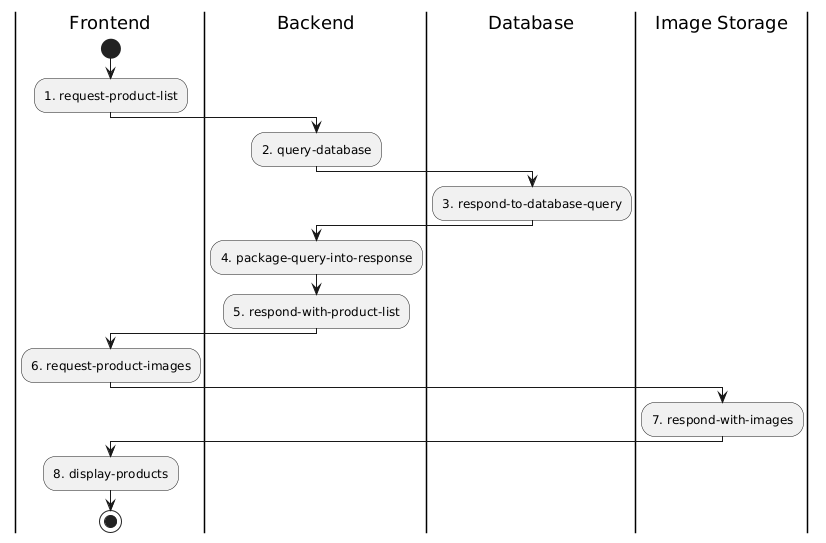
\includegraphics{images/uml_swimlane_product_list.png}

Description...


\hypertarget{__runtime_scenario_2}{%
\subsection{\textless Cart Checkout Process\textgreater{}}\label{__runtime_scenario_2}}
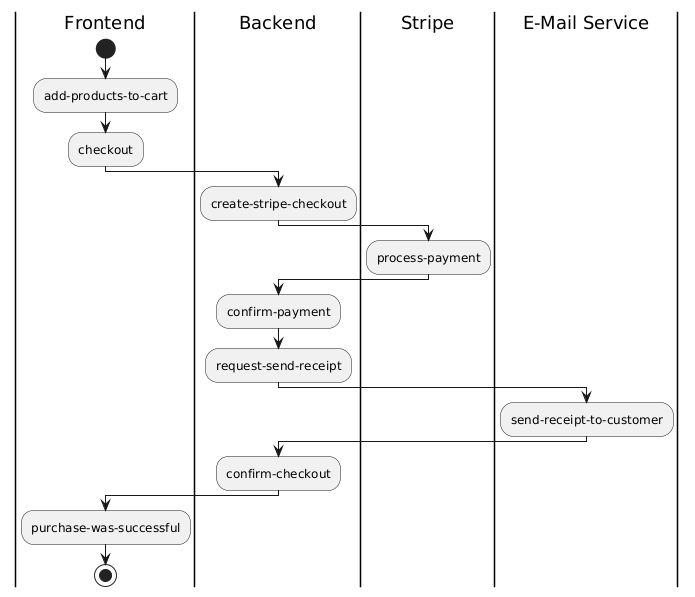
\includegraphics{images/uml_swimlane_checkout.png}

Description...

\hypertarget{__runtime_scenario_3}{%
\subsection{\textless Creating/Updating/Deleting Products in Admin Panel\textgreater{}}\label{__runtime_scenario_3}}
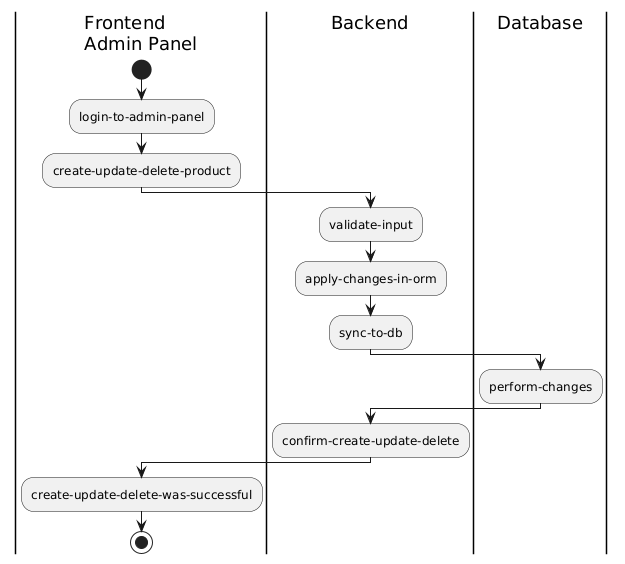
\includegraphics{images/uml_swimlane_product_create_update_delete.png}

Description...

\begin{itemize}
\item
  \emph{\textless insert runtime diagram or textual description of the
  scenario\textgreater{}}
\item
  \emph{\textless insert description of the notable aspects of the
  interactions between the building block instances depicted in this
  diagram.\textgreater{}}
\end{itemize}